\section{Results}
\label{sec:results}

\subsection{Accuracy}
\label{sec:res-acc}

\runin{Fine-tuning worked.} On the six train room recordings, none of which were in the fine-tuning data, fine-tuning raised Parakeet's word recall from 63.8\% to 72.3\%, a paired gain of 8.5 points (95\% interval 5.0 to 10.8; Figure~\ref{fig:accuracy}c). Recall on Nixon's own words rose from 49.3\% to 64.9\% and on short replies from 32.2\% to 46.7\%, while WER fell from 39.0\% to 31.3\%.

\runin{The corpus beat Whisper on held-out data.} On the 165 FRUS conversations, the corrected layer recovered 76.1\% of reference words, against 69.2\% for Whisper alone (Table~\ref{tab:main}, Figure~\ref{fig:accuracy}). Of the 6.9-point gain (interval 6.3 to 7.7), 4.5 points came from fine-tuned Parakeet and 2.4 from correction. The corpus was more accurate than Whisper on 160 of the 165 conversations. The gap between the two recognizers was largest on Nixon's own words, which Parakeet v5 recovered at 71.6\% and Whisper at 63.6\%, and on short replies, at 50.8\% and 36.0\%. By location, the corrected layer recovered 85.6\% of words at Camp David, 83.7\% on the telephone, 76.6\% in the Oval Office, 76.5\% in the Cabinet Room and 49.3\% in the EOB (Figure~\ref{fig:accuracy}d).

\runin{Correction supplied the names.} Parakeet v5 recovered 60.2\% of names and Whisper 60.0\%. Correction raised name recall by 19.8 points, to 80.1\%, with no loss of precision: of the reference names the corrected layer displayed, 90.3\% were right, against 89.0\% for Whisper alone.

\begin{table}[t]
\centering
\caption{Accuracy of each corpus layer (\%). Train: the five train room recordings in the corpus (48,189 reference words). Test: 165 held-out FRUS conversations (351,883 reference words), with 95\% bootstrap intervals over conversations in brackets.}
\label{tab:main}
\small
\setlength{\tabcolsep}{4pt}
\begin{tabular}{@{}l ccc ccc@{}}
\toprule
 & \multicolumn{3}{c}{Train (five room recordings)} & \multicolumn{3}{c}{Test (165 FRUS conversations)} \\
\cmidrule(lr){2-4}\cmidrule(lr){5-7}
Layer & Word recall & WER & Names & Word recall & WER & Names \\
\midrule
Whisper large-v3 alone & 57.2 & 45.8 & 48.8 & 69.2 {\footnotesize[67.4, 70.7]} & 42.0 & 60.0 {\footnotesize[57.0, 62.8]} \\
Parakeet v5 alone & 72.4 & 31.3 & 73.0 & 73.7 {\footnotesize[72.0, 75.1]} & 38.1 & 60.2 {\footnotesize[57.2, 63.2]} \\
Merged (no language model) & 72.5 & 31.1 & 73.1 & 73.7 {\footnotesize[72.1, 75.2]} & 37.9 & 60.3 {\footnotesize[57.2, 63.2]} \\
Corrected & \textbf{73.9} & \textbf{29.6} & \textbf{81.2} & \textbf{76.1} {\footnotesize[74.5, 77.6]} & \textbf{35.1} & \textbf{80.1} {\footnotesize[77.3, 82.5]} \\
\bottomrule
\end{tabular}
\end{table}

\begin{figure}[t]
  \centering
  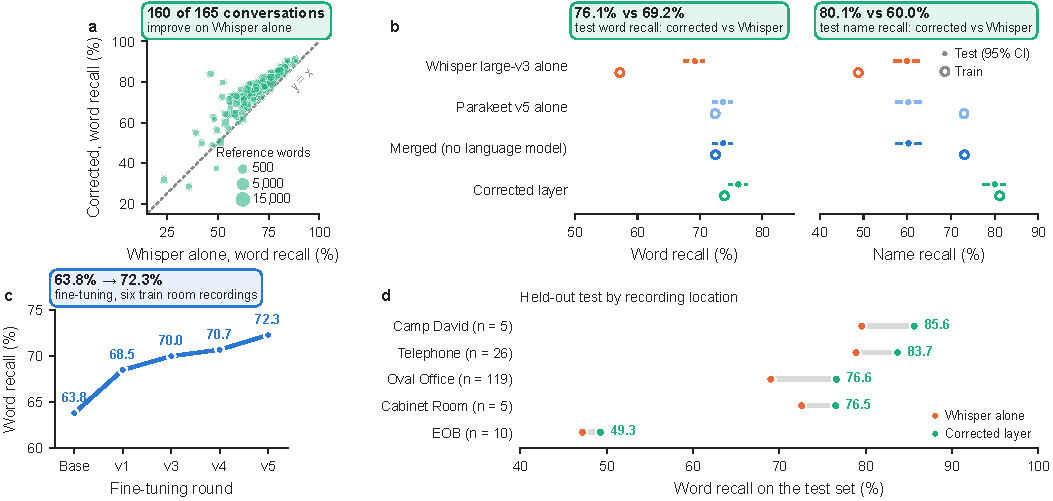
\includegraphics[width=\linewidth]{figures/fig2_accuracy.pdf}
  \caption{Accuracy. \textbf{a},~Word recall of each of the 165 held-out FRUS conversations, Whisper alone against the corrected layer (marker size: reference words). \textbf{b},~Word and name recall of each layer on the test set (filled, 95\% intervals) and the five train room recordings in the corpus (open). \textbf{c},~Fine-tuning: pooled word recall on the six train room recordings, by round. \textbf{d},~Test word recall by recording location, Whisper alone and corrected.}
  \label{fig:accuracy}
\end{figure}

\subsection{Artifacts of single-model transcription}
\label{sec:res-artifacts}

\runin{Whisper alone looped, dropped speech and wrote over silence} (Figure~\ref{fig:artifacts}). Its output contained 2,613 repetition loops, the same words written over and over, in 1,463 conversations (55,140 words); Parakeet v5 produced 105 loops and the released corrected layer 265. When run in batches with WhisperX \citep{bain2023whisperx}, the configuration of earlier machine transcriptions of the tapes \citep{fine2026easynixon}, Whisper also discarded speech: wherever WhisperX wrote nothing for 20 seconds or more, Parakeet still transcribed speech. These 3,973 stretches held 5.2\% of Parakeet's words in those conversations, and in 2,869 of them Parakeet wrote at least 60 words a minute, a rate that only real speech produces. Over NARA's muted withdrawals, Whisper wrote 1,882 words in 422 conversations, typically \enquote{you} every 30 seconds, while Parakeet wrote 131 words over the same silence. Across the corpus, Whisper also wrote 987 stock phrases such as \enquote{thank you for watching}. No word inside a muted passage was kept in the release. Each recognizer also heard words that the other missed, and both were therefore kept in the corpus.

\begin{figure}[t]
  \centering
  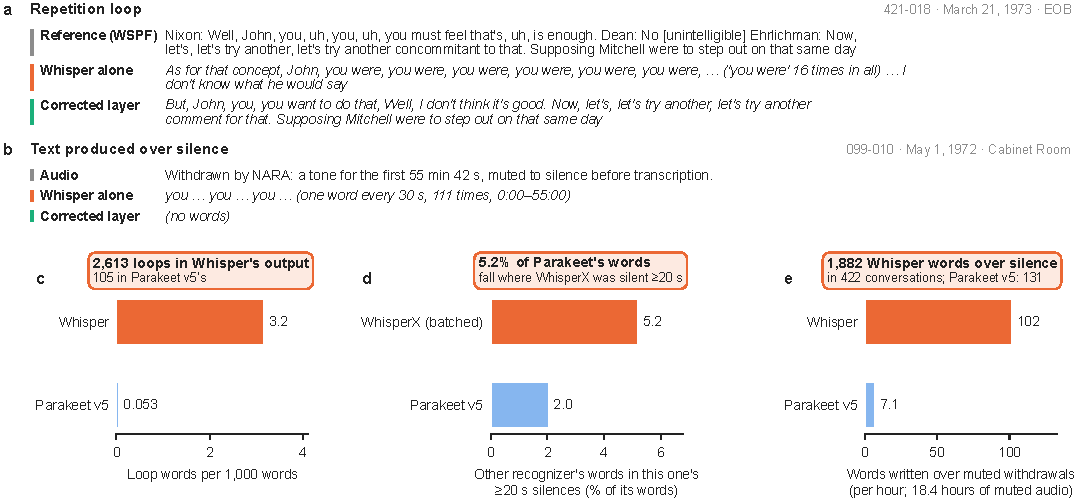
\includegraphics[width=\linewidth]{figures/fig3_artifacts.pdf}
  \caption{Artifacts of Whisper-only transcription, from the corpus's own Whisper layer. \textbf{a},~A repetition loop (\conv{421-018}): Whisper repeated \enquote{you were} sixteen times and lost Ehrlichman's turn; the corrected layer recovered it. \textbf{b},~Text over silence (\conv{099-010}): across a 55-minute withdrawal, muted before transcription, Whisper wrote \enquote{you} every 30 seconds; the corrected layer held no words. \textbf{c},~Loop words per 1,000 words, whole corpus. \textbf{d},~Dropped speech: the other recognizer's words that fell in this one's silences of 20 seconds or more (WhisperX: the batched fifth). \textbf{e},~Words written over muted withdrawals per hour of muted audio.}
  \label{fig:artifacts}
\end{figure}

\subsection{What the second reading and the correction added}
\label{sec:res-correct}

On the Test set, at least one recognizer was right on 79.5\% of reference words, 6.0 points more than Parakeet alone on the same words, and correction recovered 2.4 of those points. \textbf{The second reading drove the gain.} On the five train room recordings in the corpus, correction gained 405 reference words when given Parakeet's text alone, 564 when Whisper's readings were added and 712 when low-confidence words were also marked; before the corpus run, 340 edits helped and 20 hurt. \textbf{Same-day context corrected across recordings.} On April 9, 1971, Parakeet's \machine{want Dr. Burns, uh, Marjorie Burns? I'm pleased to call} (\conv{476-021}) was corrected to \machine{Find Dr. Burns, Arthur Burns, I placed a call}, the words of the telephone recording of the same moment (\conv{001-061}); the author confirmed both by ear. \textbf{Edits cited their evidence.} Of the corrected names in the Test set, 42.8\% cited Whisper's reading and 34.8\% the subject log; only 4.6\% cited the model's own knowledge.

\subsection{Speakers}
\label{sec:res-speakers}

On the 130 Test conversations outside the classifier's training data (220,664 aligned words), the classifier named the speaker of 68.4\% of words, and \textbf{92.4\% of named words carried the speaker named in the FRUS transcript}. For the fourteen voices it was trained on, the figure was 95.9\%: 94.9\% for Nixon over 78,305 named words and 97.5\% for Kissinger over 50,743 (Figure~\ref{fig:corpus}c). Its cross-validated balanced accuracy, the average of its accuracy on each voice, was 87.2\%.
